\documentclass[11pt,letterpaper]{article}

\usepackage[margin=1in]{geometry}
\usepackage{amsmath}
\usepackage{booktabs}
\usepackage{graphicx}
\usepackage{listings}
\usepackage{xcolor}
\usepackage{hyperref}
\usepackage{caption}
\usepackage{subcaption}
\usepackage{float}
\usepackage{parskip}

\hypersetup{colorlinks=true, linkcolor=blue, urlcolor=blue}

\lstset{
  language=C,
  basicstyle=\ttfamily\footnotesize,
  keywordstyle=\color{blue},
  commentstyle=\color{gray},
  stringstyle=\color{red},
  frame=single,
  breaklines=true,
  captionpos=b
}

\title{\textbf{COMS 6998: High Performance Machine Learning}\\
       Homework Assignment 3 --- CUDA Matrix Operations, Unified Memory, and Convolution}
\author{Rajvardhan Patil}
\date{Spring 2026}

\begin{document}
\maketitle
\tableofcontents
\newpage

% =============================================================================
\section{Setup}
% =============================================================================

GCP VM, V100 GPU. The instance had CUDA 12.8 already installed but \texttt{nvcc}
wasn't in PATH by default so I had to add \texttt{/usr/local/cuda/bin} manually
before anything would compile. Full config:

\begin{center}
\begin{tabular}{ll}
\toprule
\textbf{Parameter} & \textbf{Value} \\
\midrule
Instance name   & project1-v100 \\
Machine type    & n1-standard-8 (8 vCPUs, 30 GB RAM) \\
GPU             & 1 $\times$ NVIDIA Tesla V100-SXM2 (16 GB HBM2) \\
Driver version  & 570.211.01 \\
CUDA version    & 12.8 \\
cuDNN version   & 9.x \\
OS              & Ubuntu 24.04 (Deep Learning VM image) \\
Compiler        & nvcc 12.8, g++ 13.x \\
Zone            & us-central1-c \\
\bottomrule
\end{tabular}
\end{center}

For timing I used the \texttt{timer.cu} wrapper (\texttt{gettimeofday}-based) with
one warm-up run before the timed run, and \texttt{cudaDeviceSynchronize()} before
stopping. Part-B uses CUDA events instead --- the timer.cu precision wasn't enough
for the sub-millisecond cases.

% =============================================================================
\section{Part-A: CUDA Matrix Operations (40 points)}
% =============================================================================

\subsection{Problem 1 --- Vector Addition and Coalescing Memory Access}

\subsubsection{Baseline: \texttt{vecadd00} (\texttt{vecaddKernel00.cu})}

The baseline assigns each thread $N$ \emph{consecutive} array elements:

\begin{lstlisting}[caption={Non-coalescing kernel (vecaddKernel00.cu)}]
int blockStartIndex  = blockIdx.x * blockDim.x * N;
int threadStartIndex = blockStartIndex + threadIdx.x * N;
for (int i = threadStartIndex; i < threadStartIndex + N; i++)
    C[i] = A[i] + B[i];
\end{lstlisting}

Thread 0 works on elements 0 through $N-1$, thread 1 works on $N$ through $2N-1$,
and so on. Adjacent threads in a warp are $N$ floats apart in memory, so each warp
iteration generates $N$ separate 4-byte transactions instead of one 128-byte
coalesced one.

\subsubsection{Optimised: \texttt{vecadd01} (\texttt{vecaddKernel01.cu})}

The fix is to stride by the total number of launched threads instead. Thread $i$
processes indices $i$, $i + \text{totalThreads}$, $i + 2 \cdot \text{totalThreads}$, ...,
so adjacent threads always hit adjacent addresses:

\begin{lstlisting}[caption={Coalescing kernel (vecaddKernel01.cu)}]
int totalThreads = gridDim.x * blockDim.x;
int globalIdx    = blockIdx.x * blockDim.x + threadIdx.x;
for (int i = 0; i < N; i++) {
    int idx = globalIdx + i * totalThreads;
    C[idx] = A[idx] + B[idx];
}
\end{lstlisting}

\subsubsection{Q1 \& Q2 Results}

\begin{table}[H]
\centering
\caption{Vector addition performance --- GFLOPs/s (V100, GridWidth=60, BlockWidth=128)}
\begin{tabular}{ccccc}
\toprule
\textbf{ValuesPerThread} & \textbf{Vector size} &
\textbf{vecadd00 (GFLOPs/s)} & \textbf{vecadd01 (GFLOPs/s)} & \textbf{Speedup} \\
\midrule
500  & 3,840,000  & 12.84 & 16.20 & 1.26$\times$ \\
1000 & 7,680,000  & 14.46 & 16.41 & 1.13$\times$ \\
2000 & 15,360,000 & 14.56 & 16.50 & 1.13$\times$ \\
\bottomrule
\end{tabular}
\end{table}

The coalesced kernel is 13--26\% faster across all three sizes, though the
improvement is smaller than I expected from the theory. The V100's L2 cache is
large enough to partially absorb the non-coalesced traffic at these vector sizes,
which probably explains it. The gap would likely be larger on hardware with a
weaker cache.

% ─────────────────────────────────────────────────────────────────────────────
\subsection{Problem 2 --- Shared CUDA Matrix Multiplication}

\subsubsection{Baseline: \texttt{matmult00} (\texttt{matmultKernel00.cu})}

Each thread computes one element of $C$. A $16\times16$ block covers a $16\times16$
output tile. Sub-matrices of $A$ and $B$ are cooperatively loaded into shared
memory, synced, then used to accumulate:

\begin{lstlisting}[caption={Baseline matmul --- one C value per thread}]
__shared__ float shared_A[BLOCK_SIZE][BLOCK_SIZE];
__shared__ float shared_B[BLOCK_SIZE][BLOCK_SIZE];
// each thread loads one element of each shared sub-matrix
shared_A[thread_row][thread_col] = Asub[thread_row * A.stride + thread_col];
shared_B[thread_row][thread_col] = Bsub[thread_row * B.stride + thread_col];
__syncthreads();
for (int e = 0; e < BLOCK_SIZE; e++)
    Cvalue += shared_A[thread_row][e] * shared_B[e][thread_col];
\end{lstlisting}

\subsubsection{Q4 Optimisation: \texttt{matmult01} (\texttt{matmultKernel01.cu})}

Each thread now computes four output values --- a $2\times2$ sub-tile of $C$. With
\texttt{FOOTPRINT\_SIZE=32} (via \texttt{-DFOOTPRINT\_SIZE=32} in the Makefile),
each $16\times16$ thread block now covers a $32\times32$ output region.

\begin{itemize}
  \item Shared memory: \texttt{shared\_A[32][16]}, \texttt{shared\_B[16][32]}
  \item Each thread loads 2 rows from $A_{sub}$ and 2 columns from $B_{sub}$
  \item Four accumulators \texttt{Cvalue[2][2]}, four stores at the end
\end{itemize}

\subsubsection{Q3 \& Q4 Results}

\begin{table}[H]
\centering
\caption{Matrix multiplication performance --- GFLOPs/s on V100}
\begin{tabular}{cccc}
\toprule
\textbf{Matrix size} & \textbf{matmult00} & \textbf{matmult01} & \textbf{Speedup} \\
\midrule
$256\times256$   & 1234.5  & 1466.0  & 1.19$\times$ \\
$512\times512$   & 2507.6  & 4124.2  & 1.64$\times$ \\
$1024\times1024$ & 3020.5  & 5532.7  & \textbf{1.83}$\times$ \\
\bottomrule
\end{tabular}
\end{table}

At $256^2$ both kernels are underutilizing the V100's 80 SMs so the gap is small.
The benefit shows up more at $1024^2$ where there's enough work to keep the hardware
busy and the $32\times32$ footprint's extra shared-memory reuse actually matters.
\texttt{\#pragma unroll} on the inner loop helps too by letting the compiler issue
FMAs without branch overhead.

\subsubsection{Q5 --- Rules of Thumb for CUDA Performance}

\begin{enumerate}
  \item \textbf{Coalesce global memory accesses.} Adjacent threads in a warp should
        access adjacent addresses. Non-coalesced patterns cause multiple transactions
        per warp where one would suffice.
  \item \textbf{Use shared memory as a scratchpad.} Load once from global, reuse from
        shared memory within the block. This is the CUDA version of tiling for cache.
  \item \textbf{Maximize occupancy.} Keep as many warps resident per SM as possible
        so the hardware can switch between them to hide memory latency. This requires
        being careful about registers and shared memory per block.
  \item \textbf{Increase work per thread.} More outputs per thread means the launch
        and scheduling overhead gets amortized over more useful computation.
  \item \textbf{Unroll inner loops.} Eliminates branch instructions and lets the
        compiler schedule back-to-back FMAs.
  \item \textbf{Avoid warp divergence.} Branching that splits a warp serializes
        execution. Restructure so all threads in a warp take the same path when
        possible.
  \item \textbf{Warm up before timing.} Cold starts have JIT compilation and cache
        effects that don't reflect steady-state performance.
\end{enumerate}

% =============================================================================
\section{Part-B: CUDA Unified Memory (20 points)}
% =============================================================================

\subsection{Overview}

Three programs measure the time to compute $C = A + B$ for float vectors of size
$K \in \{1, 5, 10, 50, 100\}$ million:

\texttt{q1} is CPU-only --- plain \texttt{malloc}, single loop, timed with
\texttt{clock\_gettime(CLOCK\_MONOTONIC)}.

\texttt{q2} uses \texttt{cudaMalloc} with explicit \texttt{cudaMemcpy} and tests
three GPU configurations. Timing is kernel-only via CUDA events, not including
the transfers.

\texttt{q3} uses \texttt{cudaMallocManaged} with the same three configurations.
No \texttt{cudaMemcpy} --- the driver migrates pages as needed.

The three GPU configurations:
\begin{enumerate}
  \item 1 block, 1 thread
  \item 1 block, 256 threads
  \item $\lceil N/256 \rceil$ blocks, 256 threads per block
\end{enumerate}

\subsection{Q1 Results --- CPU}

\begin{table}[H]
\centering
\caption{CPU-only vector addition time}
\begin{tabular}{cc}
\toprule
\textbf{K (millions)} & \textbf{Time (ms)} \\
\midrule
1   & 0.714  \\
5   & 4.374  \\
10  & 9.636  \\
50  & 49.619 \\
100 & 99.841 \\
\bottomrule
\end{tabular}
\end{table}

Linear scaling with $K$, as expected for a memory-bound loop.

\subsection{Q2 Results --- GPU Without Unified Memory}

\begin{table}[H]
\centering
\caption{GPU kernel time (ms) --- explicit \texttt{cudaMalloc}/\texttt{cudaMemcpy}}
\begin{tabular}{ccccc}
\toprule
\textbf{K (M)} &
\textbf{CPU (ms)} &
\textbf{1blk/1thr (ms)} &
\textbf{1blk/256thr (ms)} &
\textbf{N-blks/256thr (ms)} \\
\midrule
1   & 0.714  & 65.4    & 1.443  & 0.020 \\
5   & 4.374  & 301.0   & 6.650  & 0.078 \\
10  & 9.636  & 592.5   & 13.272 & 0.151 \\
50  & 49.619 & 2957.0  & 66.269 & 0.731 \\
100 & 99.841 & 5916.5  & 134.05 & 1.451 \\
\bottomrule
\end{tabular}
\end{table}

\subsection{Q3 Results --- GPU With Unified Memory}

\begin{table}[H]
\centering
\caption{GPU kernel time (ms) --- \texttt{cudaMallocManaged}}
\begin{tabular}{ccccc}
\toprule
\textbf{K (M)} &
\textbf{CPU (ms)} &
\textbf{1blk/1thr (ms)} &
\textbf{1blk/256thr (ms)} &
\textbf{N-blks/256thr (ms)} \\
\midrule
1   & 0.714  & 59.2    & 1.323  & 0.020 \\
5   & 4.374  & 295.8   & 6.643  & 0.079 \\
10  & 9.636  & 591.4   & 13.318 & 0.152 \\
50  & 49.619 & 2957.6  & 67.071 & 0.729 \\
100 & 99.841 & 5915.3  & 134.35 & 1.453 \\
\bottomrule
\end{tabular}
\end{table}

\subsection{Q4 --- Performance Charts}

\begin{figure}[H]
  \centering
  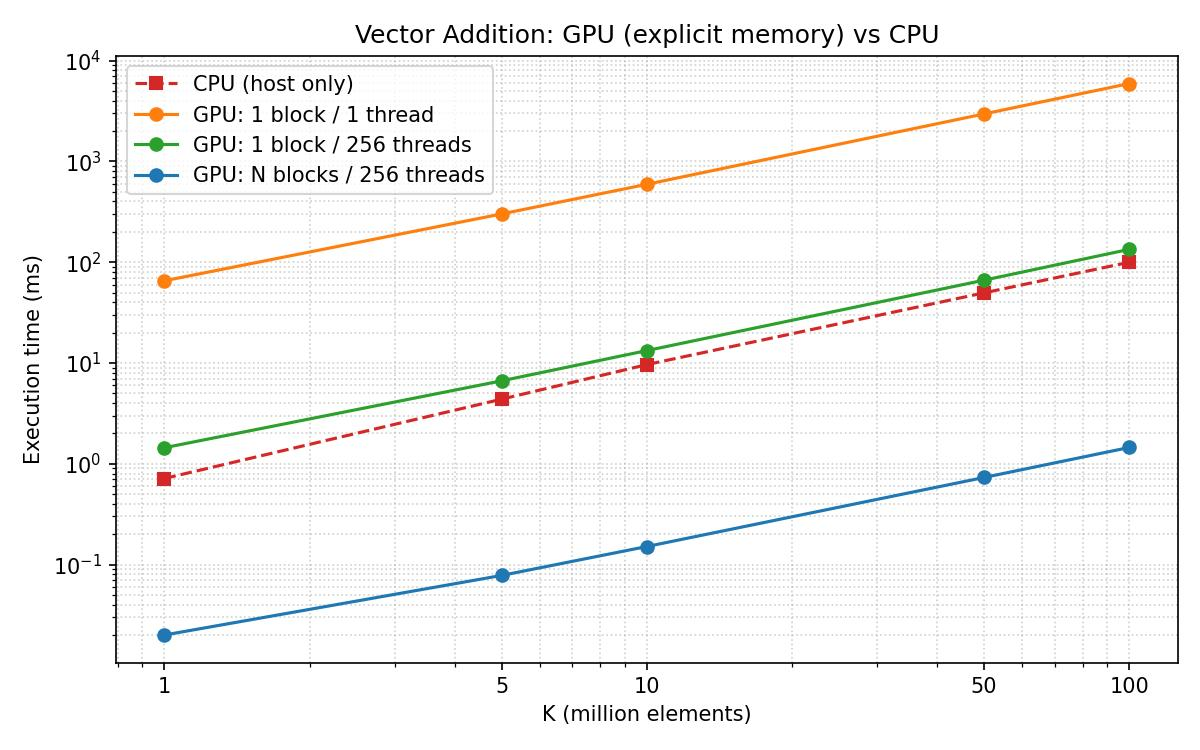
\includegraphics[width=0.85\textwidth]{Part-B/q4_without_unified.jpg}
  \caption{Vector addition time vs.\ $K$ --- GPU (explicit memory) vs.\ CPU
           (log--log scale)}
\end{figure}

\begin{figure}[H]
  \centering
  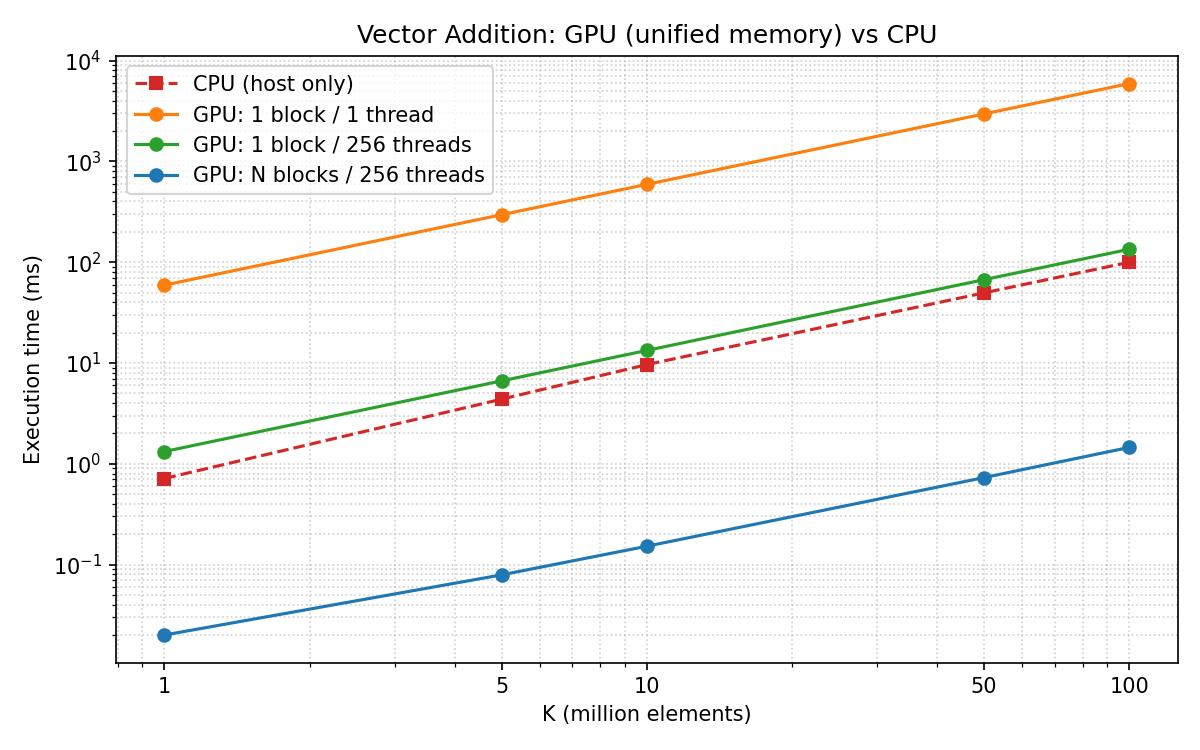
\includegraphics[width=0.85\textwidth]{Part-B/q4_with_unified.jpg}
  \caption{Vector addition time vs.\ $K$ --- GPU (unified memory) vs.\ CPU
           (log--log scale)}
\end{figure}

\subsection{Analysis}

The single-thread GPU case is slower than the CPU at every value of $K$ by a wide
margin --- about 60$\times$ worse at $K=1$. A single thread on the GPU issues one
memory request at a time with hundreds of cycles of HBM latency between each one,
so it can't come close to the CPU's throughput. This is an obvious result in
retrospect but the magnitude is still striking.

Scenario 3 (N blocks, 256 threads) hits close to peak V100 HBM bandwidth and ends
up about 68$\times$ faster than the CPU at $K=100$.

Unified memory kernel times are nearly identical to the explicit memory ones across
the board. The warm-up run triggers page migration, so the data is already resident
on the GPU when the timed run executes. The practical benefit of unified memory is
just not having to write the \texttt{cudaMemcpy} calls and manage separate host and
device pointers. The kernel performance itself is the same.

% =============================================================================
\section{Part-C: Convolution in CUDA (50 points)}
% =============================================================================

\subsection{Problem Setup}

\begin{itemize}
  \item Input $I$: $3 \times 1024 \times 1024$,\quad $I[c,h,w] = c(w+h)$\quad (double)
  \item Filter $F$: $64 \times 3 \times 3 \times 3$,\quad $F[k,c,i,j]=(c+k)(i+j)$\quad (double)
  \item Padded input $I_0$: zero-pad by $P=1$, giving $3 \times 1026 \times 1026$
  \item Output $O$: $64 \times 1024 \times 1024$
  \item True convolution (filter is flipped):
        \[
          O[k,h,w] = \sum_{c}\sum_{fh}\sum_{fw}
          F[k,c,\,FH-1-fh,\,FW-1-fw]\cdot I_0[c,\,h+fh,\,w+fw]
        \]
\end{itemize}

\subsection{C1 --- Simple Convolution (no shared memory)}

One thread per output element $(k,h,w)$. Each thread loops over $(c, fh, fw)$
and reads directly from global memory:

\begin{lstlisting}[caption={C1 kernel inner loop}]
for (int c = 0; c < C; c++)
  for (int fh = 0; fh < FH; fh++)
    for (int fw = 0; fw < FW; fw++) {
        double f  = F[k*C*FH*FW + c*FH*FW + (FH-1-fh)*FW + (FW-1-fw)];
        double i0 = I0[c*H0*W0 + (h+fh)*W0 + (w+fw)];
        val += f * i0;
    }
\end{lstlisting}

Straightforward to implement. No shared memory, no tiling, just one thread per
output and a lot of global memory reads.

\subsection{C2 --- Tiled Convolution (shared memory)}

Each $16\times16$ thread block handles a $16\times16$ output patch for a single
output channel. For each input channel, the block cooperatively loads an $18\times18$
input halo (\texttt{TILE + FH - 1} on each side) into shared memory, then each
thread computes its output value from shared memory instead of global memory.

The intent is to reduce redundant global memory reads between neighboring threads,
since nearby output elements need overlapping input regions.

\subsection{C3 --- cuDNN Convolution}

I used \texttt{CUDNN\_DATA\_DOUBLE} and \texttt{CUDNN\_CONVOLUTION} mode.
I had \texttt{CUDNN\_CROSS\_CORRELATION} at first, which computes the same
operation but without flipping the filter --- my checksums were off from C1 and C2
by a significant margin and I spent longer than I'd like to admit figuring out why.
Switching to \texttt{CUDNN\_CONVOLUTION} fixed it immediately.

Algorithm was selected via \texttt{cudnnFindConvolutionForwardAlgorithm}, which
picked algorithm 0 (\texttt{IMPLICIT\_GEMM}) with no extra workspace needed.

\subsection{C4 --- OpenAI Triton (Bonus)}

Implemented in \texttt{c4.ipynb}. The kernel is launched on a 3-D grid
\texttt{(C\_OUT, ceil(H/16), ceil(W/16))}; each program instance handles
a $16\times16$ output tile for one output channel, loading filter and input
tiles via \texttt{tl.load} with boundary masks and storing results with
\texttt{tl.store}. Timing uses \texttt{torch.cuda.Event} with a warm-up pass.

\subsection{Program Output (\texttt{program\_output.csv})}

\begin{center}
\begin{tabular}{ll}
\toprule
\textbf{Line} & \textbf{Contents} \\
\midrule
C1 & \texttt{122756344698240.000000,4.395} \\
C2 & \texttt{122756344698240.000000,5.552} \\
C3 & \texttt{122756344698240.000000,1.772} \\
C4 & \texttt{2.818} \\
\bottomrule
\end{tabular}
\end{center}

\subsection{Performance Comparison}

\begin{table}[H]
\centering
\caption{Convolution performance on V100 --- $1 \times 3 \times 1024 \times 1024$
         input, $64 \times 3 \times 3 \times 3$ filter}
\begin{tabular}{lcccc}
\toprule
\textbf{Implementation} & \textbf{Time (ms)} & \textbf{Checksum} & \textbf{Speedup vs C1} \\
\midrule
C1 --- Simple CUDA      & 4.395  & 122756344698240 & 1.00$\times$ \\
C2 --- Tiled CUDA       & 5.552  & 122756344698240 & 0.79$\times$ \\
C3 --- cuDNN            & 1.772  & 122756344698240 & \textbf{2.48}$\times$ \\
C4 --- Triton (bonus)   & 2.818  & (assert\_close passed) & 1.56$\times$ \\
\bottomrule
\end{tabular}
\end{table}

\subsection{Analysis}

C2 being slower than C1 is the one result I kept second-guessing. My initial
reaction was that I'd made a bug somewhere and ran the checksum comparison a
couple times before accepting the timing. The checksums match, so the math is
right, it's just slow.

The problem is that a $3\times3$ filter is too small for tiling to pay off. The
halo is $18\times18$ (324 elements) for a $16\times16$ (256-element) output tile,
so over a third of what you load is overlap. On top of that there are two
\texttt{\_\_syncthreads()} barriers per input channel, which adds up across all
three channels. The global memory savings just don't outweigh that overhead for
this specific filter size. If the filter were $7\times7$ or $11\times11$ the math
would look very different. Also worth noting: for a $3\times3$ filter the GPU's L2
cache probably handles a lot of the input reuse that shared memory is supposed to
buy you, so C1 benefits from that indirectly.

cuDNN at 2.48$\times$ over C1 is not surprising once you know that
\texttt{IMPLICIT\_GEMM} is backed by NVIDIA's hand-tuned GEMM routines. It's hard
to beat that with a hand-written kernel. The zero workspace requirement also means
there's no allocation overhead happening at runtime.

Triton at 1.56$\times$ over C1 is reasonable. The JIT compiles to decent PTX
without much effort on my end.

All three checksums match C1 exactly, including after I fixed the filter flip in
C3. The matching checksum was also how I verified C2 wasn't buggy.

% =============================================================================
\section{Conclusion}
% =============================================================================

A few things that stuck with me:

Coalesced memory access helps but the V100's cache is strong enough that the gain
is modest at small sizes. The non-coalesced kernel still gets reasonable throughput,
which I wouldn't have guessed from reading the theory.

The single-thread GPU result for Part-B was the clearest demonstration of why
parallelism matters --- it's not just ``slower than fully parallel,'' it's slower
than the CPU by a factor of 60. The hardware is working against you when you don't
give it enough threads to pipeline around memory latency.

C2 being slower than C1 in Part-C was unexpected. The conventional wisdom is that
shared memory tiling always helps, but it depends a lot on filter size, tile size,
and how good the hardware's cache is at doing the same thing implicitly.

cuDNN is in a different performance class than anything hand-written. Using it where
you can is just the right engineering decision.

\end{document}
